\documentclass[a4paper,12pt]{report}
\usepackage{graphicx}
\begin{document}
\title{Trabajo Practico $N^o 1$}
\author{Electronica III}
\author{Grupo 2}
\date{\today} %ver si dejar la de today o poner fecha fija que sea August 2018
\pagenumbering{arabic}

\maketitle

\section{Excercise 1: Resolution and Range of a Fixed-Point Binary Representation}

\subsection{What is the Fixed-Point Binary Representation}
A fixed-point number has an integer part and a fractional part separated by a decimal point with a fixed position, as shown below:
$$ (Integer Part).(Fractional Part)$$
The integer part is formed by $n$ bits and the fractional part is formed by $m$ bits.
$$ (bit \#1\ \ \ bit \#2\ \ \ ...\ \ \ bit \#n).(bit \#1\ \ \ bit \#2\ \ \ ...\ \ \ bit \#m)$$

\subsection{What is Resolution and Range}
\subsubsection{Resolution}
The resolution of a number using the fixed point representation is the smallest unit that can be handled with it.
Given a fixed-point number with $m$ fractional bits, the resolution is $2^-m$.
\subsubsection{Range}
The range is the difference between the biggest value that can be obtained with the fixed-point representation of a number with $n$ bits in the integer part and with $m$ bits in the fractional part, and the smallest number that can be represented.
%ver de poner la ecuacion matematica que permite obtener el range.

\subsection{Making Use of this Program}
\subsubsection{Input}
Three arguments must be entered through Command Line, separated by one space:
\begin{enumerate}
\item  1 (indicating that the numeric representation of the binary number is signed) or 0 (indicating that the representation is unsigned).
\item $n$: A possitive integer (indicating the number of bits corresponding to the integer part of the number, which is the part before the decimal point).
\item  $m$: A possitive integer (indicating the number of bits corresponding to the fractional part of the number, which is the part after the decimal point).
\end{enumerate}
For example: "0 1 1"

\subsubsection{Output}
The result of this program is the resolution and range of the number that has $n$ digits in the integer part and $m$ digits in the fractional part.

\begin{figure}[h!]
\centering
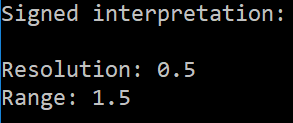
\includegraphics[scale=1]{ejemploOutput}
\caption{Output corresponding to the input $"0\ 1\ 1"$.}
\label{image output}
\end{figure}

\subsection{Testing the Program}


% beginners guide to latex:
% http://www.docs.is.ed.ac.uk/skills/documents/3722/3722-2014.pdf

% fixed point mathematics:
%http://fileadmin.cs.lth.se/cs/Education/EDA075/notes/mgh_appA_fixed.pdf


\end{document}
